%----------------------------------------------------------------------------------------
%	The MIT License (MIT)
%	Copyright (c) 2021 Jitin Nair
%	Copyright (c) 2025 CORGNET Yoann

% Modified by Yoann CORGNET in 2025 to include customizations.

%----------------------------------------------------------------------------------------
%	DOCUMENT DEFINITION
%----------------------------------------------------------------------------------------

% article class because we want to fully customize the page and not use a cv template
\documentclass[a4paper,10pt]{article}

%----------------------------------------------------------------------------------------
%	FONT
%----------------------------------------------------------------------------------------

% % fontspec allows you to use TTF/OTF fonts directly
% \usepackage{fontspec}
% \defaultfontfeatures{Ligatures=TeX}

% % modified for ShareLaTeX use
% \setmainfont[
% SmallCapsFont = Fontin-SmallCaps.otf,
% BoldFont = Fontin-Bold.otf,
% ItalicFont = Fontin-Italic.otf
% ]
% {Fontin.otf}

%----------------------------------------------------------------------------------------
%	PACKAGES
%----------------------------------------------------------------------------------------
\usepackage{url}
\usepackage{parskip} 	

%other packages for formatting
\RequirePackage{color}
\RequirePackage{graphicx}
% photo outside public/: ../images/ when compiling from public/, images/ from the repo root
\graphicspath{{../images/}{images/}}
\usepackage[usenames,dvipsnames]{xcolor}
\usepackage[scale=0.9]{geometry}

%tabularx environment
\usepackage{tabularx}

%for lists within experience section
\usepackage{enumitem}

% centered version of 'X' col. type
\newcolumntype{C}{>{\centering\arraybackslash}X} 

%to prevent spillover of tabular into next pages
\usepackage{supertabular}
\usepackage{tabularx}
\newlength{\fullcollw}
\setlength{\fullcollw}{0.47\textwidth}

%custom \section
\usepackage{titlesec}				
\usepackage{multicol}
\usepackage{multirow}
\usepackage{tcolorbox}

%CV Sections inspired by: 
%http://stefano.italians.nl/archives/26
\titleformat{\section}{\Large\scshape\raggedright}{}{0em}{}[\titlerule]
\titlespacing{\section}{0pt}{8pt}{8pt}

%Setup hyperref package, and colours for links
\usepackage[unicode, draft=false]{hyperref}
\definecolor{linkcolour}{rgb}{0,0.2,0.6}
\hypersetup{colorlinks,breaklinks,urlcolor=linkcolour,linkcolor=linkcolour}

%for social icons
\usepackage{fontawesome5}

%debug page outer frames
%\usepackage{showframe}


% job listing environments
\newenvironment{jobshort}[2]
    {
    \begin{tabularx}{\linewidth}{@{}l X r@{}}
    \textbf{#1} & \hfill &  #2 \\[3.75pt]
    \end{tabularx}
    }
    {
    }

\newenvironment{joblong}[2]
    {
    \begin{tabularx}{\linewidth}{@{}l X r@{}}
    \textbf{#1} & \hfill &  #2 \\[3.75pt]
    \end{tabularx}
    \begin{minipage}[t]{\linewidth}
    \begin{itemize}[nosep,after=\strut, leftmargin=1em, itemsep=2.5pt,label=--]
    }
    {
    \end{itemize}
    \end{minipage}    
    }

% joblong with a school logo in a fixed-width column, so titles stay aligned
\newenvironment{joblogo}[4]
    {
    \begin{tabularx}{\linewidth}{@{}p{2.5cm} X r@{}}
    \raisebox{-0.3\height}{\includegraphics[height=#1]{#2}} & \textbf{#3} & #4 \\[3.75pt]
    \end{tabularx}
    \begin{minipage}[t]{\linewidth}
    \begin{itemize}[nosep,after=\strut, leftmargin=1em, itemsep=2.5pt,label=--]
    }
    {
    \end{itemize}
    \end{minipage}
    }

%----------------------------------------------------------------------------------------
%	BEGIN DOCUMENT
%----------------------------------------------------------------------------------------
\begin{document}

% non-numbered pages
\pagestyle{empty} 

%----------------------------------------------------------------------------------------
%	TITLE
%----------------------------------------------------------------------------------------

\begin{minipage}{0.15\textwidth} % Photo area
    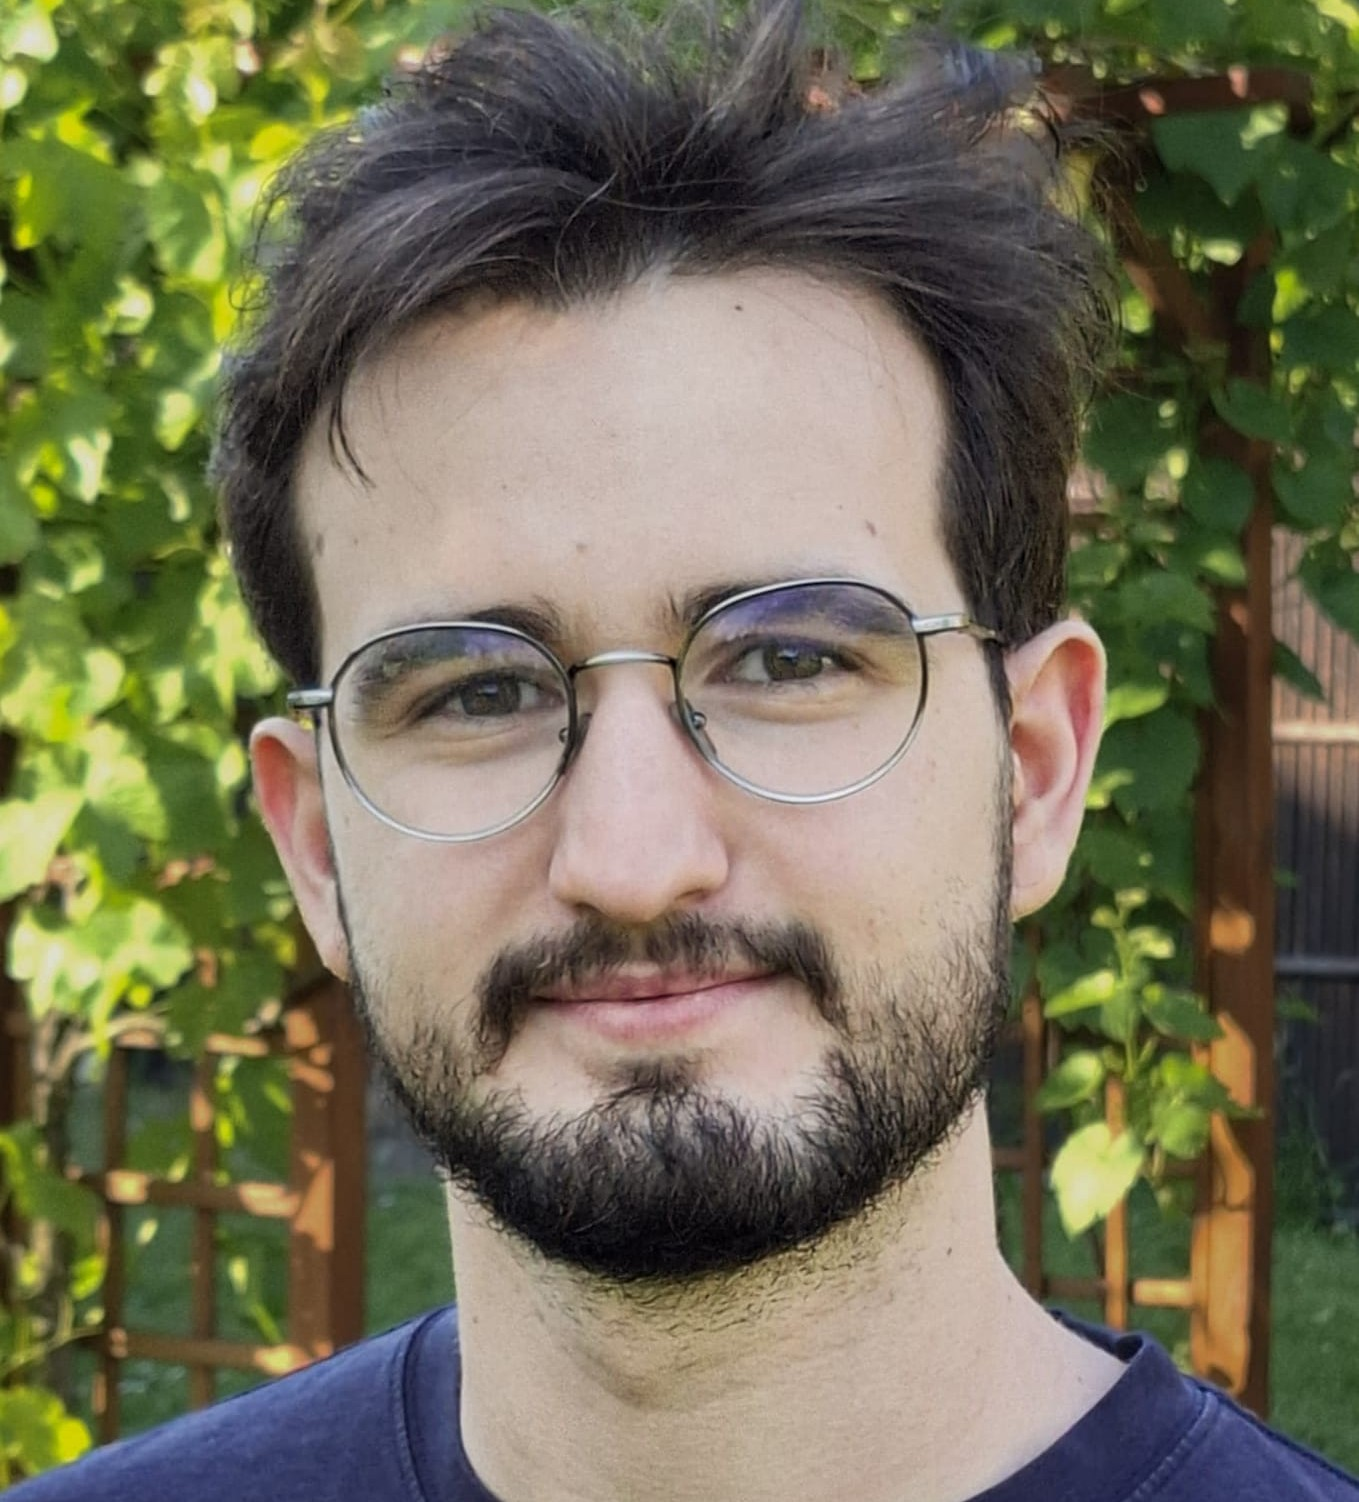
\includegraphics[width=\textwidth]{tronche.jpg}
\end{minipage} \hfill
\begin{minipage}{0.83\textwidth} % Text area (name, contact, etc.)
    \Huge{Yoann CORGNET} \\[3pt]
    \large{Software Engineering student} \\
    \large{Seeking a 6-month end-of-studies internship (May - December 2027)} \\
    \large{Target roles: Software Engineer or DevOps Engineer} \\[7.5pt]
    \href{https://www.linkedin.com/in/yoann-corgnet/}{\raisebox{-0.05\height}\faLinkedin\ linkedin.com/in/yoann-corgnet} \ $|$ \
    \href{https://github.com/Yoann-CORGNET}{\raisebox{-0.05\height}\faGithub\ github.com/Yoann-CORGNET} \\
    \href{mailto:yoann.corgnet.04@gmail.com}{\raisebox{-0.05\height}\faEnvelope \ yoann.corgnet.04@gmail.com} \ $|$ \
    \href{tel:+33768229430}{\raisebox{-0.05\height}\faMobile \ +33.7.68.22.94.30}
\end{minipage}


%----------------------------------------------------------------------------------------
%	ABOUT
%----------------------------------------------------------------------------------------

\section{About}
I am an engineering student (ESIEA, double degree with CentraleSupélec) and have been the technical lead of a SaaS \mbox{in production.} I am looking for an end-of-studies internship in software: architecture, governance, microservices, distributed systems, cloud, DevOps.


%----------------------------------------------------------------------------------------
%	SKILLS
%----------------------------------------------------------------------------------------
\section{Skills}
\begin{tabularx}{\linewidth}{@{}l X@{}}
Languages  &  \normalsize{JavaScript, TypeScript, Java, Python, C}\\
Frameworks  &  \normalsize{Next.js, Vue.js, Java Spring, Django}\\
DevOps \& Cloud  &  \normalsize{Git, GitHub Actions, CI/CD, Google Cloud}\\
Spoken languages  &  \normalsize{French (native), English (TOEIC 970: C1)}\\
\end{tabularx}

%----------------------------------------------------------------------------------------
% EXPERIENCE SECTIONS
%----------------------------------------------------------------------------------------

\section{Professional Experience}

\begin{joblong}{NerionSoft - Full-Stack Developer}{Sep. 2025 - Present}
    \item Technical lead of Hestia, a SaaS booking engine for independent hotels
    \item TypeScript, Next.js, PostgreSQL; hexagonal architecture; CI/CD with GitHub Actions, Neon + Vercel previews
    \item Integration of the Apaleo PMS (OAuth2, webhooks) and Apaleo Pay payments; app certified on the Apaleo Store
\end{joblong}

%Projects
\section{Projects}

\begin{joblong}{Undrive - 4th-year project}{Sep. 2025 - Feb. 2026}
    \item Gamified mobile app encouraging public transport use through a rewards system
    \item Designed the CI/CD infrastructure with Terraform on GCP, Cloud Run deployment and GitHub workflow management
    \item Developed the Django backend API, integrated Python microservices and a PostgreSQL + PostGIS database
\end{joblong}

\begin{joblong}{StockElec - Silver medal (2nd-year project)}{2023 - 2024}
    \item Inventory management web app for ESIEA's electronics lab
    \item Agile development, including gathering the client's requirements
    \item Frontend: Quasar (Vue.js), Tailwind CSS, interactive analytics dashboard
    \item Backend: RESTful API in Java Spring, MySQL database, all containerised with Docker
\end{joblong}

%----------------------------------------------------------------------------------------
%	EDUCATION
%----------------------------------------------------------------------------------------

\section{Education}
\begin{joblogo}{0.95cm}{logo-centralesupelec.png}{CentraleSupélec Double Degree - Software Science track}{2026 - 2027}
    \item Software engineering: advanced programming (C++), testing, static analysis, continuous integration, agile methods
    \item Systems: operating systems, concurrent and distributed systems, distributed algorithms and models
    \item Foundations: advanced algorithms, logic and deductive systems, semantics and language processing
\end{joblogo}

\begin{joblogo}{0.55cm}{logo-esiea.pdf}{ESIEA Engineering Degree (MSc) - Software Engineering major}{Expected 2027}
    \item Systems (C), mobile (Flutter) and full-stack (Vue.js, Spring) development: SOLID, application design, architecture
    \item Systems administration: virtualisation, containerisation
    \item Data Science \& AI: SQL/NoSQL, data analysis, Machine Learning, AI
\end{joblogo}

\begin{joblogo}{0.45cm}{logo-uqac.pdf}{UQAC Double Degree - Bachelor's in Computer Science}{2024 - 2025}
    \item Cybersecurity: vulnerability detection (network/web), attack graphs (Nmap, Nessus), forensics
    \item Big Data and AI: multivariate linear regression, decision trees, clustering, neural networks (MLP, CNN)
\end{joblogo}

\end{document}
